\documentclass[a4paper,english,12pt,bibliography=totoc]{scrreprt}

\usepackage[T1]{fontenc} %immer
\usepackage[utf8]{inputenc} %am
\usepackage{babel} %Anfang

\usepackage{enumitem} %Aufzählungen verändern

%Gleichungen verwenden
\usepackage{newtxtext}
\usepackage{amsmath}
\usepackage{amssymb}
\usepackage{mathptmx}
%\usepackage{txfonts}
\usepackage{wrapfig}
\usepackage{graphicx} % To include graphics
\usepackage{listings}% code blocks
\usepackage[most]{tcolorbox}

%Querverweise
\usepackage{varioref} %immer
\usepackage{hyperref} %in dieser
\usepackage{cleveref} %Reihenfolge

\usepackage{booktabs} %schönere Tabellen
\usepackage{siunitx} %SI-Einheiten
\usepackage{tabularx} %Tabellen mit flexiblen Spalten	

\usepackage{graphicx} %Grafiken verwenden

\usepackage[backend=biber,style=numeric]{biblatex}
\addbibresource{main.bib} 

\usepackage{lipsum} %Blindtext
\usepackage{subcaption}
\usepackage{afterpage}
\usepackage[headsepline]{scrlayer-scrpage} %Paket für Kopfzeilen
\usepackage{afterpage}
\usepackage{float}
\automark[subsection]{section}

\pagestyle{scrheadings}
\ihead{} % oben links
\chead{\leftmark} % oben Mitte
\ohead{} % oben rechts
\cfoot{\pagemark} % unten Mitte
\automark[section]{section} % Modified line

% Zu volle hboxen korrigieren
\tolerance 1414
\hbadness 1414
\emergencystretch 1.5em
\hfuzz 0.3pt
\widowpenalty=10000
\vfuzz \hfuzz
\raggedbottom

%Informationen über das Dokument
\date{\today}


\begin{document}


\begin{titlepage}
	\centering
	
\includegraphics[width=0.8\textwidth]{logo_uulm_sw}
	
	\vspace{1cm}
	\LARGE Laboratory Module for Master Programs
	\Huge \textbf{Biophysics Lab Course}
	
	\vspace{1cm}
	\Large Experiment:

	\Huge \textbf{Superresolution Microscopy}
	
	\vspace{15mm}
	\Large Performed on 10.07.2024
	
	\vspace{5mm}
	\LARGE Group 8
	
	\vspace{1cm}
	\Large
	\begin{tabular}{rcl}
	\textbf{Haiyang Zhang} & and & \textbf{Nicolae Turcan}\\
	\href{mailto:student.1@uni-ulm.de}{haiyang.zhang@uni-ulm.de} & & \href{mailto:student.2@uni-ulm.de}{nicolae.turcan@uni-ulm.de}
	\end{tabular}
	
	\vspace{7mm}
	Supervisor: Mara Hofmann
	
	\vfill
	\begin{tabular}{p{50mm}@{\hspace{5cm}}p{50mm}}
	\hrulefill & \hrulefill \\
	%\centering Haiyang Zhang  & \centering Nicolae Turcan
	\end{tabular}
	
	\vspace{5mm}
	\normalsize \raggedright
	We hereby confirm that we have elaborated the present work independently and have detailed knowledge of the entire contents.
\end{titlepage}



\tableofcontents

\chapter{Introduction}
\label{cha:Introduction}

Super-resolution fluorescence microscopy techniques, such as Single-Molecule Localization Microscopy (SMLM), offer significant advantages for visualizing cellular structures beyond the classical diffraction limit. This lab course focused on utilizing advanced imaging techniques to study DNA origami structures and the nuclear pore complex (NPC) in U2OS cells.

Fluorescence microscopy is a widely used tool for investigating the distribution and interaction of proteins within cells however, its resolution is fundamentally limited by diffraction, which restricts the minimal resolvable distance between two fluorescent emitters. This limitation can be overcome using super-resolution techniques like SMLM, which achieved higher resolution through the precise localization of individual fluorescent molecules over time and establishing a center for the gaussian function of Intensity(Figure~\ref{fig:smlsm}).


\begin{figure}[H]
            \centering
            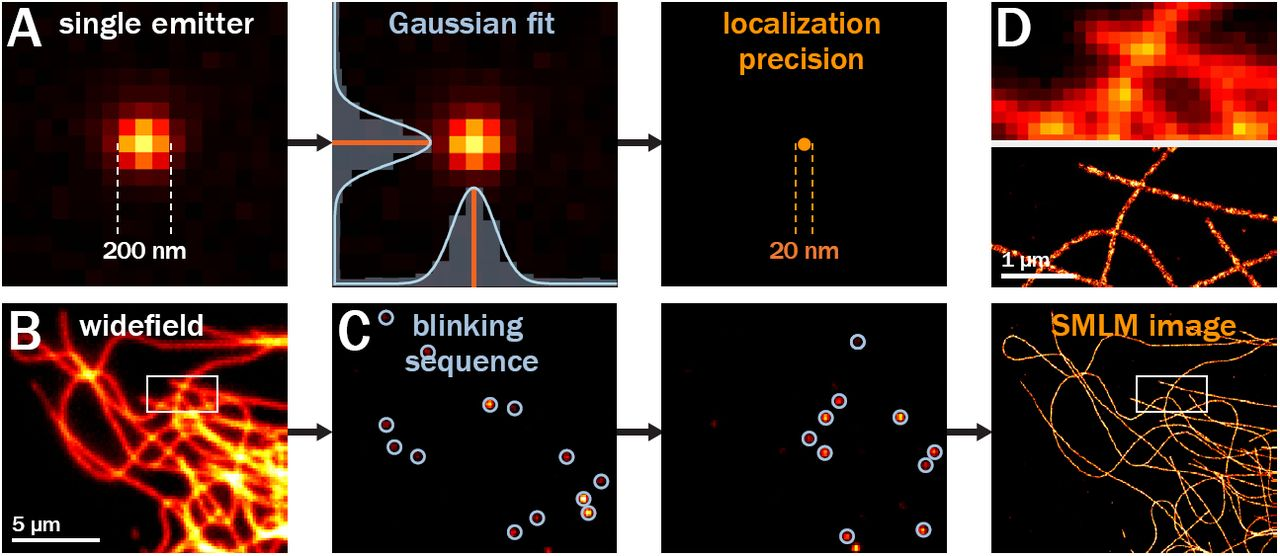
\includegraphics[width=1\linewidth]{Principle of Single Molecule Localization Microscopy (SMLM).png }
            \caption{Principle of Single Molecule Localization Microscopy \cite{Jimenez2019}}
            \label{fig:smlsm}
\end{figure}
 

DNA origami nanorulers were imaged using DNA-PAINT, a method that leveraged the transient binding of fluorescently labeled oligonucleotides to complementary strands on the target structure (Figure~\ref{fig:dnapaint}). This technique reduced photobleaching and allowed for multiplexing, enabling the simultaneous imaging of multiple targets.
\begin{figure}[H]
        \centering
        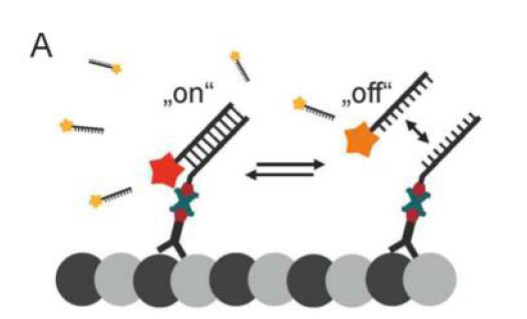
\includegraphics[width=0.9\linewidth]{dnapaint.png}
        \caption{DNA Paint Principle \cite{Sauer2017-hu}}
        \label{fig:dnapaint}
    \end{figure}

    


Additionally, the course examined the NPC, a crucial cellular structure involved in selective molecular transport between the nucleus and cytoplasm. In our experiments, Nup96 proteins within the NPC were labeled with a red fluorescent dye, Alexa 647, via an antibody that bound to an attached GFP molecule, facilitating their visualization using the STORM technique (Figure~\ref{fig:comples}).

\begin{figure}[h]
    \centering
    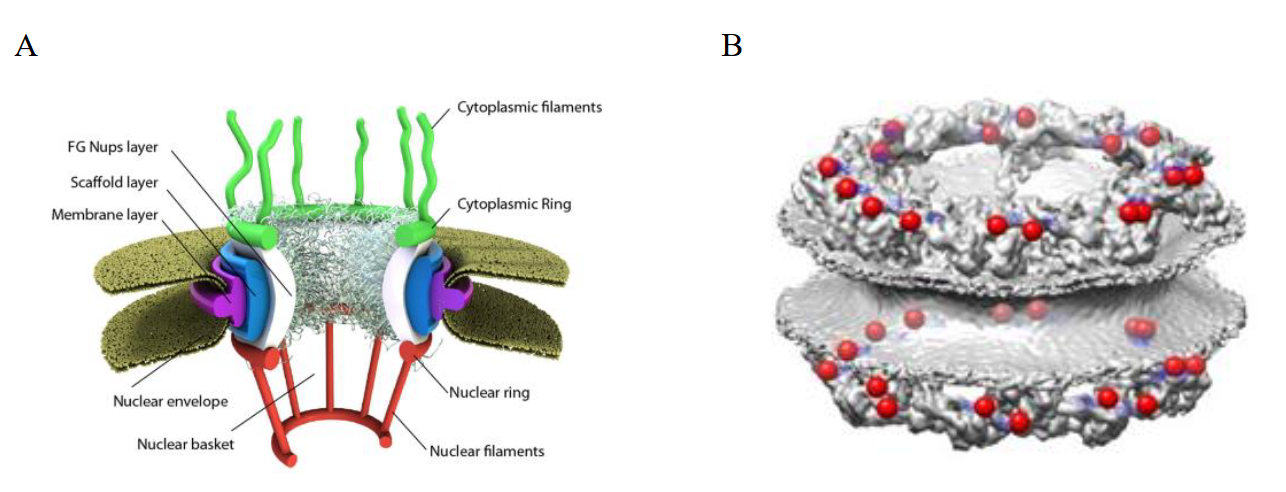
\includegraphics[width=0.9\textwidth]{ncp.png}
    \caption{Nuclear pore complex. A) Schematic of the nuclear pore complex. B) EM density of the nuclear pore complex with C termini of Nup96 indicated in red. \cite{Thevathasan2019}}
    \label{fig:comples}
\end{figure}

\chapter{Characterize the GATTAquant nanoruler using DNA PAINT method}

\section{Experiment}
The experiment focused on characterizing the GATTAquant nanoruler trough the DNA-PAINT technique. The transient binding events generated localized fluorescence signals, which were used to reconstruct a super-resolution image with nanometer accuracy.

We were provided with a commercially prepared slide containing DNA origami structures immobilized on a glass surface. We imaged it with the SMLM setup  that was built on a vibration isolation optical table.
A 638-nm diode laser was coupled into a single-mode optical fiber, collimated, and directed to the objective using a 45° angled mirror. The lens focusing on the back-focal plane of the objective allowed switching between epi-illumination and TIRF/ HALO-illumination. A dichroic mirror reflected the excitation light to the objective and transmitted the fluorescent signal towards the detection part.

The emitted fluorescence was imaged on an sCMOS camera with a tube lens, after blocking undesired wavelengths with a bandpass filter. The setup also included an autofocus utility with an IR laser, a position-sensitive detector, and a piezo-actuator for drift compensation which were sadly inoperative and couldn´t be used.




%the measured distances between features in the image are compared to the known distances of the reference sample. Any discrepancies can indicate the need for adjustments in the calibration or imaging system. Repeating the measurement with multiple reference samples or using different regions of the same sample can further validate the effective pixel size.By accurately determining the effective pixel size, precise measurements of nanoscale structures in subsequent experiments can be achieved, ensuring the reliability of the super-resolution microscopy data.

\subsection{GATTAquant nanoruler characterization}

%Explain what we used for the experiment(TIRF, HALO), the change of the exposure time, analyze the movie and get rid of the drift using reference dots.
The process of using DNA origami as a nanoruler for super-resolution microscopy involves several steps required  to determine spatial resolution.

First, DNA origami nanorulers with known distances between docking strands were provided by GATTAQuant. These structures serve as precise calibration standards. The sample measures 160 nm with fluorscent spost every 80nm immobilized on a glass surface, ensuring stable imaging conditions.

\begin{figure}[h] % 'r' for right, and width of the figure
  \centering
  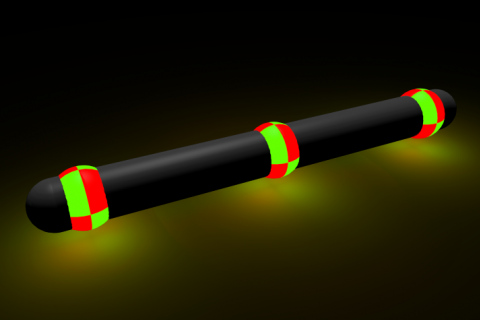
\includegraphics[width=0.4\textwidth]{image_manager__product_images_thumbnail_dna_origami_based_dna_paint_80rg_nanoruler_for_super-resolution_microscopy.png} % Replace 'example-image' with your figure file
  \caption{Gattaquant Nanoruler}
  \label{fig:example}
\end{figure}

Using the DNA-PAINT technique, transient binding of fluorescently labeled strands to the complementary docking strands on the nanoruler is achieved. This method allows sparse activation of fluorophores, fluorescence images are acquired using again the super-resolution microscope equipped with an sCMOS camera. The imager strands, labeled with a fluorescent dye, interact with the docking strands on the DNA origami, producing a series of localized fluorescence signals.

These signals are analyzed to reconstruct a super-resolution image. The distances between the docking strands are measured, providing a detailed characterization of the nanoruler's spatial resolution capabilities.\\

By comparing the measured distances to the known values , the accuracy of the super-resolution microscopy setup is validated. This process ensures that the imaging system can reliably achieve nanoscale precision, essential for subsequent experiments.

\section{Results}
%The picture with three dots, and the guassian fitting of the results, Basically follow the script.

%77.0905 4.095720293455383 mean and the std of the original data
%76.81250000000001 2.804943305032108 mean and std of the fitted data
\subsection{Nanoruler}
The DNA-PAINT technique was used to image GATTAquant nanorulers, providing a detailed visualization of the spatial resolution capabilities. Figure \ref{fig:gattarulerl} shows a typical image of the nanorulers under this technique.

\begin{figure}[H]
    \centering
    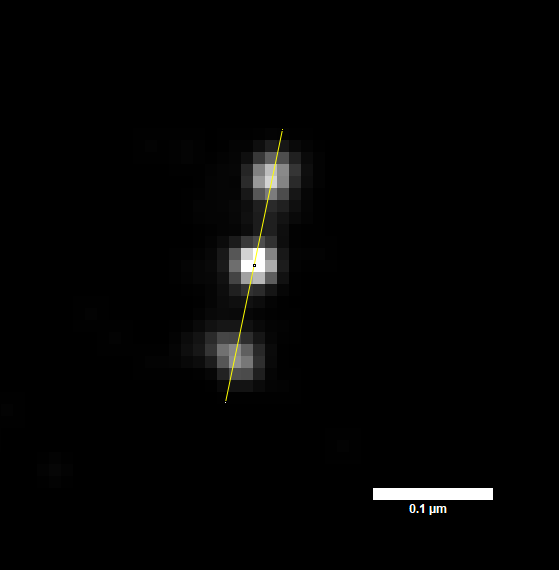
\includegraphics[width=0.35\textwidth]{Images/PAINT/triple dots.png}
    \caption{GATTAquant nanoruler.}
    \label{fig:gattarulerl}
\end{figure}
\subsection{Raw measurement nanoruler}
In the experiment, we used the movie generated from SMLM with 4800 frames, and generated the image (Figure 2.5.(d)) by ThunderSTORM plugin analysis. The nanoruler image with triple fluorescent dot could be observed. The distances between three fluorescent dots on the nanoruler were measured. As is shown in Figure 2.2, an area was selected along the triple dots of the DNA origami. The intensity (grey value in Figure 2.3) along the line was plotted, and the distances between peaks were recorded as the distances between the dots. The  The original measurements (Table \ref{tab:original_data}) showed a mean distance of 77.09 nm with a standard deviation of 4.10 nm. 

%Raw measurement of the three dots
\begin{table}[H]
    \centering
    \begin{tabular}{c|c|c|c}
    \hline
    Groups    & d$_1$ [nm] & d$_2$ [nm] & $\frac{d_1 +d_2}{2}$ [nm] \\
    \hline
     1    &  70.35&79.69 & 75.02\\
     2    &  79.88&70.02 &74.95  \\
     3    &  71.04&69.97&70.505\\
     4    &  69.22&90.29& 79.755\\
     5    &  90.48&79.80&85.14\\
     6    &  60.01&90.41 &75.21\\
     7    &  74.83&75.24 & 75.035\\
     8    &  70.06&90.01 & 80.035\\
     9    &  69.97&80.85&75.41\\
     10    & 79.69&80.00 & 79.845\\
    \hline
    \end{tabular}
    \caption{Original data of the three dots measurement. d$_1$ is the distance between dot 1 and 2. d$_2$ is the distance between dot 2 and 3. $\frac{d_1 +d_2}{2}$ is the average of the dot distance.}
    \label{tab:original_data}
\end{table}
\subsection{Gaussian fit nanoruler}
Gaussian fitting was performed on three distinct peaks using Origin's multi-peak fit functionality. This fitting process allowed for a more accurate determination of the distances between the fluorescent markers. Figure \ref{fig:gaussianfit} illustrates the results of this Gaussian fitting.

\begin{figure}[H]
    \centering
    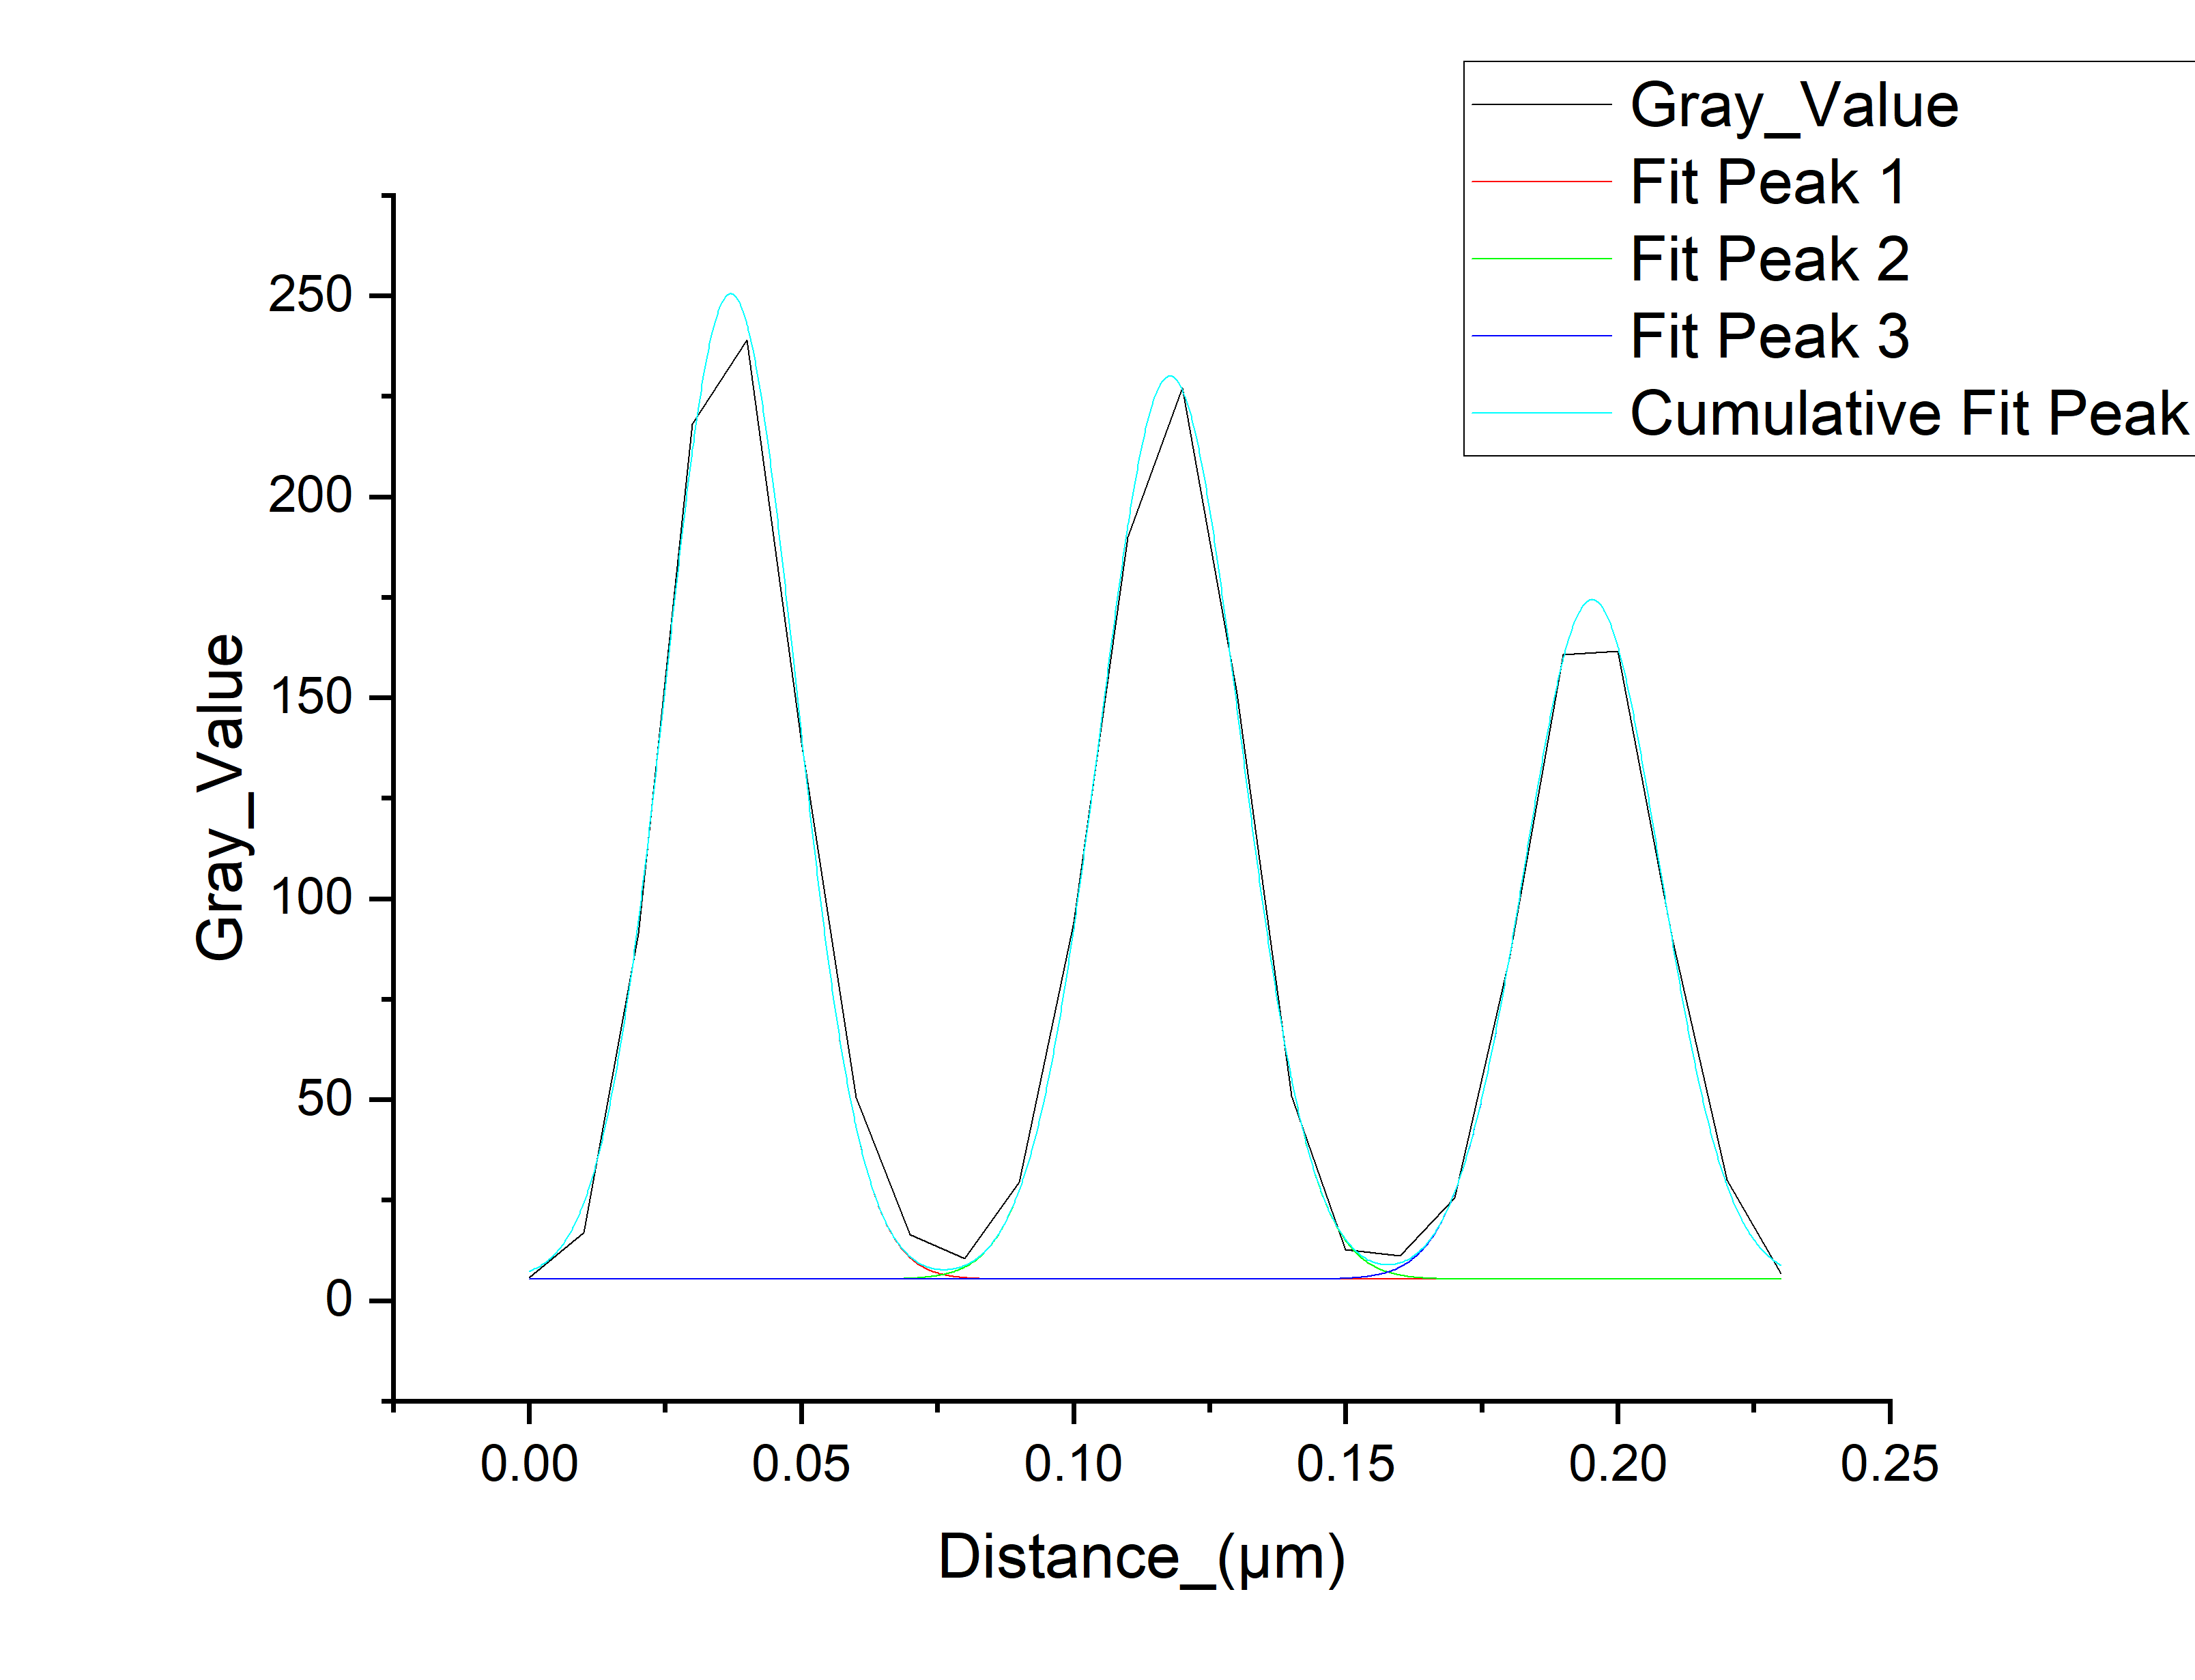
\includegraphics[width=0.65\textwidth]{Images/PAINT/Gaussian fitting example.png}
    \caption{Gaussian fit of the distance-intensity plot of the nanoruler triple dots. The intensity (grey value) along the triple dots were plotted (black line) and each peak was fitted with gaussian distribution. The distances between the dots could be determined from the distances between the fit peak 1, 2 and fit peak 2, 3.}
    \label{fig:gaussianfit}
\end{figure}

After Gaussian fitting, the mean distance was refined to 76.81 nm with a standard deviation of 2.80 nm, indicating improved precision in the localization of the fluorescent markers.(Table \ref{tab:fitted_data}).

%Gaussian fitting of the three dots
\begin{table}[H]
    \centering
    \begin{tabular}{c|c|c|c}
    \hline
    Groups    & f$_1$ [nm] & f$_2$ [nm] & $\frac{f_1 +f_2}{2}$ [nm] \\
    \hline
    1    & 71.08&78.03 &74.55\\
    2    & 81.63&70.11 &75.87\\
    3    & 71.47 &77.04 &74.255\\
    4    & 75.32 &80.77&78.045\\
    5    & 81.22&78.79&80.005\\
    6    & 66.57&83.43 &75.00\\
    7    & 69.18&76.20 &72.69\\
    8    & 75.53&87.20 &81.365\\
    9    & 143.53&10.87 &77.20\\
    10   & 80.72 &77.56 &79.14\\
    \hline
    \end{tabular}
    \caption{Fitted data of the three dots measurement. f$_1$ is the fitted distance between dot 1 and 2. f$_2$ is the fitted distance between dot 2 and 3. $\frac{f_1 +f_2}{2}$  is the average of the dot distance.}
    \label{tab:fitted_data}
\end{table}

\subsection{Drift}

During the imaging process, drift can occur due to various factors such as focus drift, sample movement, or thermal expansion/relaxation. To address this issue, we used the fiducial markers setting in ThunderSTORM for automatic drift correction because the sample contained them. This method effectively compensates for any drift, ensuring higher accuracy in the final images. Figure \ref{fig:imagewithdrift} shows an image affected by drift, while Figure \ref{fig:driftcorrected} presents the corrected image after applying the drift correction.


\begin{figure}[H]
    \centering
    \begin{subfigure}[b]{0.4\textwidth}
        \centering
        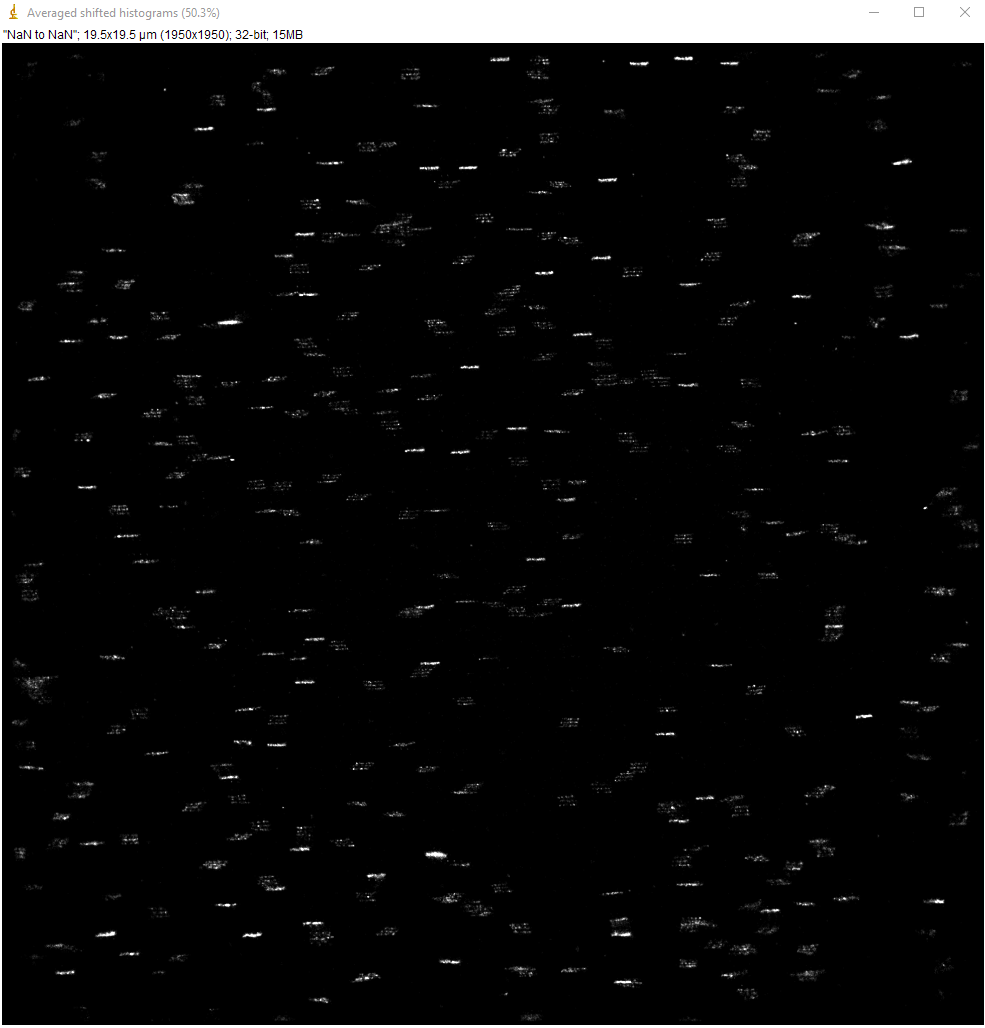
\includegraphics[width=\textwidth]{Images/PAINT/ImageWithDrift.png}
        \caption{Image with Drift}
        \label{fig:imagewithdrift}
    \end{subfigure}
    \hfill
    \begin{subfigure}[b]{0.4\textwidth}
        \centering
        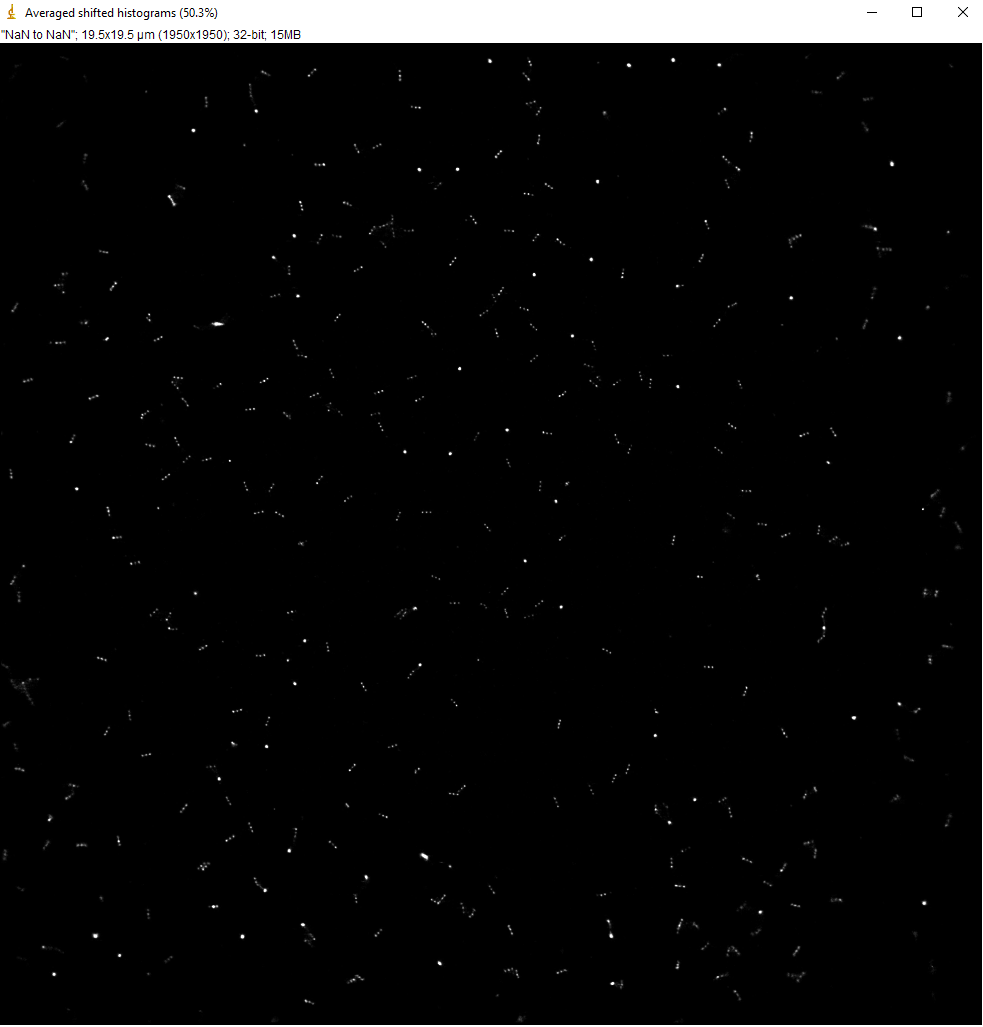
\includegraphics[width=\textwidth]{Images/PAINT/widefieldwithoutdrift.png}
        \caption{Drift corrected image}
        \label{fig:driftcorrected}
    \end{subfigure}
    \caption{}
\end{figure}

\subsection{Frames Variability}
The DNA-PAINT technique was used to image GATTAquant nanorulers under varying frame counts to analyze the impact on image reconstruction quality. Figure \ref{fig:subfigurespaint} presents the reconstructed images using different numbers of frames: 500, 2000, 3500, and 4800. This comparison allows for the evaluation of how increasing the number of frames improves the resolution and clarity of the reconstructed nanorulers.


 \begin{figure}[H]
    \centering
    \begin{subfigure}[b]{0.49\textwidth}
        \centering
        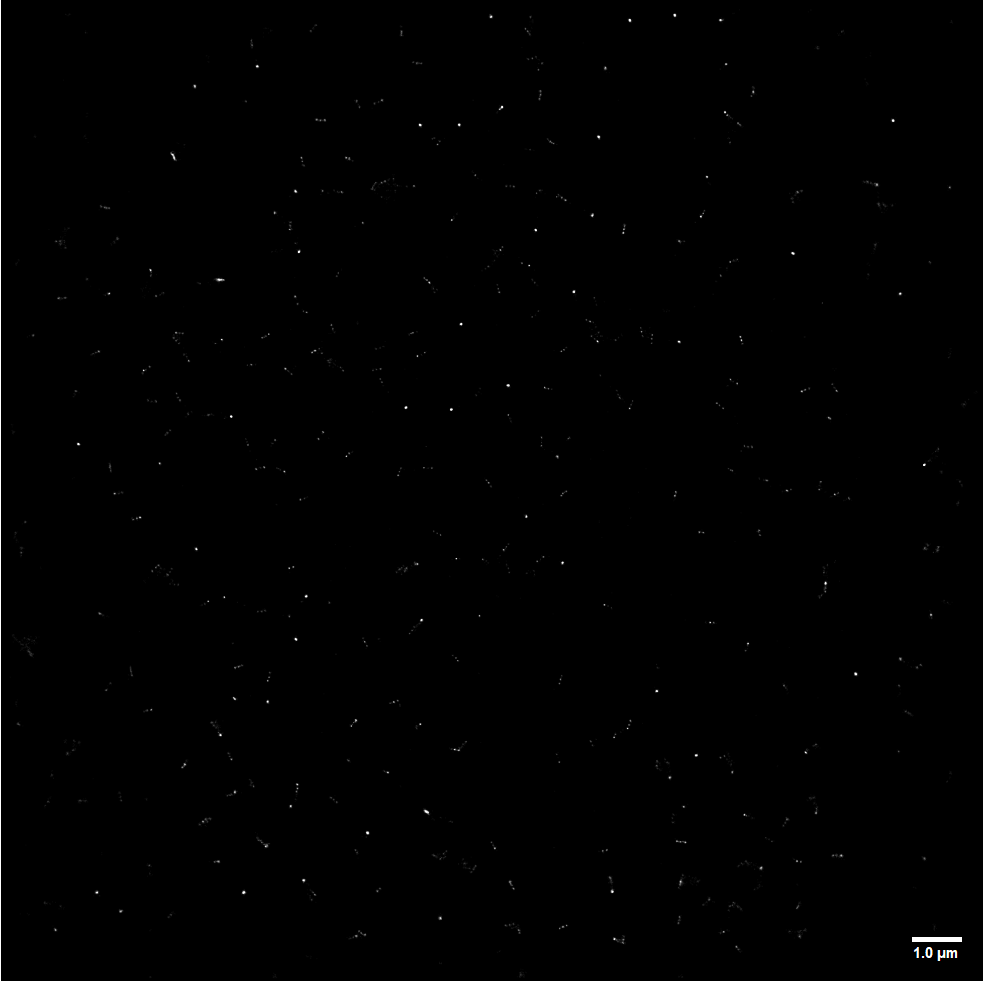
\includegraphics[width=\textwidth]{Images/PAINT/500frames.png}
        \caption{Reconstructed with 500 frames}
        \label{fig:image1}
    \end{subfigure}
    \hfill
    \begin{subfigure}[b]{0.49\textwidth}
        \centering
        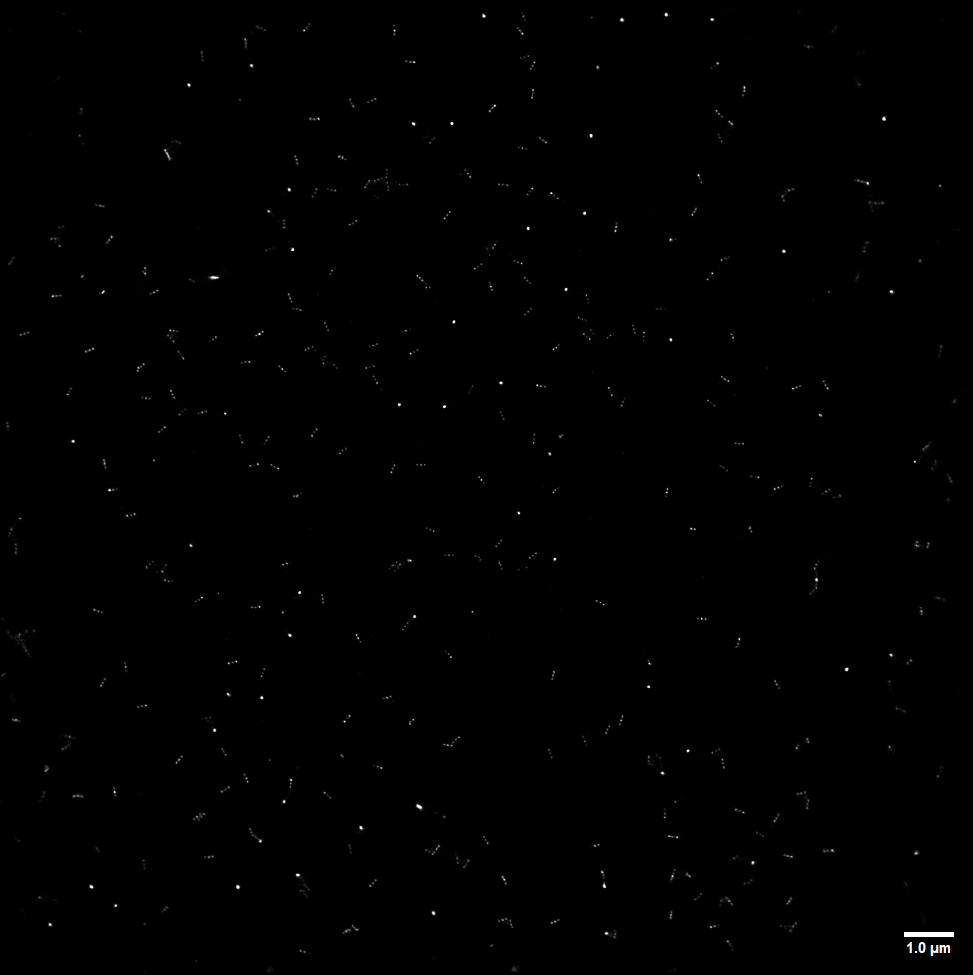
\includegraphics[width=\textwidth]{Images/PAINT/2000frames.png}
        \caption{Reconstructed with 2000 frames}
        \label{fig:image2}
    \end{subfigure}
    \vfill
    \begin{subfigure}[b]{0.49\textwidth}
        \centering
        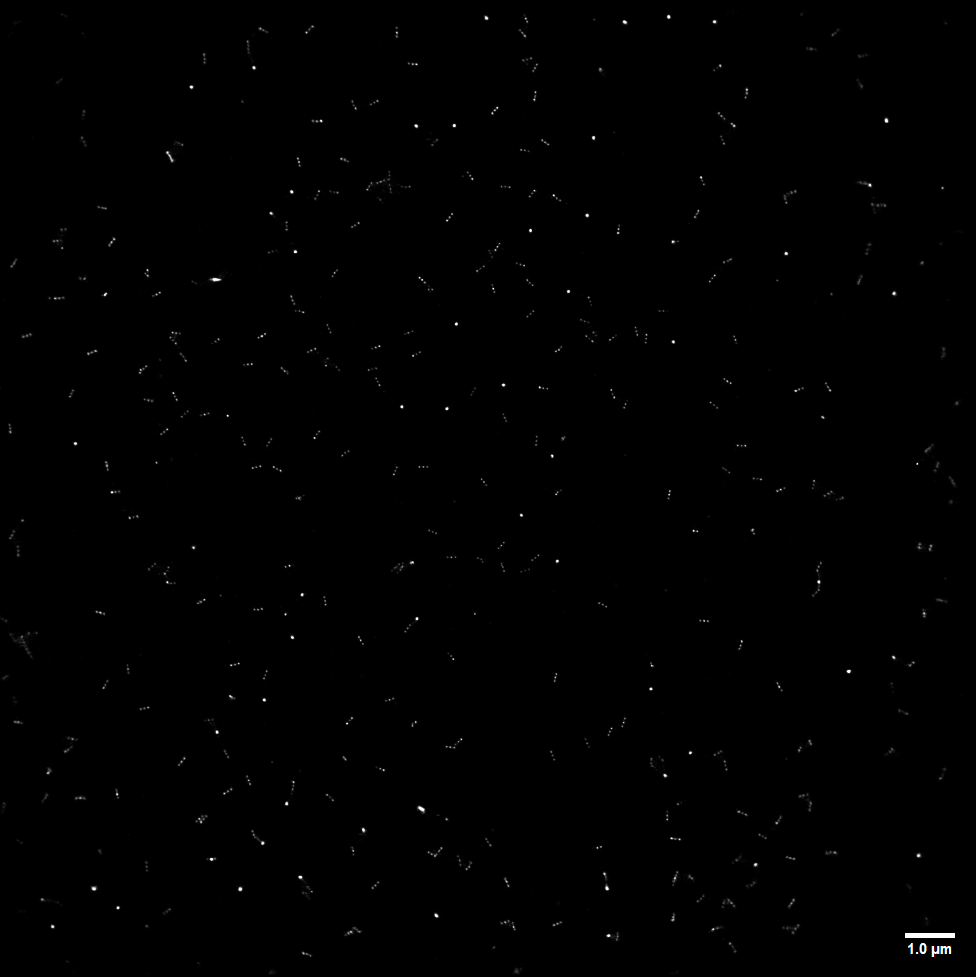
\includegraphics[width=\textwidth]{Images/PAINT/3500frames.png}
        \caption{Reconstructed with 3500 frames}
        \label{fig:image3}
    \end{subfigure}
    \hfill
    \begin{subfigure}[b]{0.49\textwidth}
        \centering
        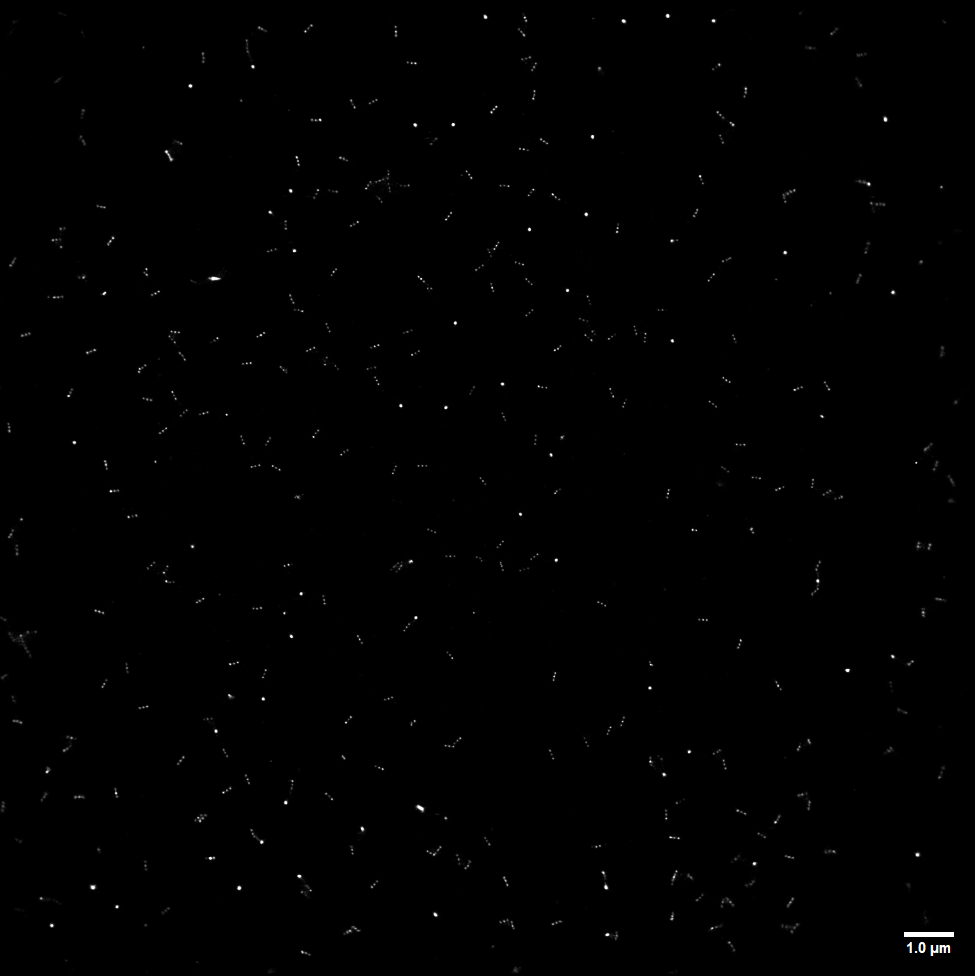
\includegraphics[width=\textwidth]{Images/PAINT/4800frames.png}
        \caption{Reconstructed with 48000 frames}
        \label{fig:image4}
    \end{subfigure}
    \caption{The  GATTAquant DNA Ruler reconstructed with different number of frames.(a), (b) and (c) are all reconstructed with 5 bins}
    \label{fig:subfigurespaint}
\end{figure}

These results demonstrate the capability of DNA-PAINT to achieve high localization precision, validating the nanoruler's effectiveness as a calibration standard for super-resolution microscopy. The DNA-PAINT technique was used to image GATTAquant nanorulers under varying frame counts to shows the increase in reconstructied image quality. 

\section{Discussion}
% Preciesion of the results, Any imporovment in methods?
The analysis of the GATTAquant Nanoruler using DNA-PAINT demonstrated the power of super-resolution microscopy in resolving structures beyond the diffraction limit. Our measurements yielded an average distance of 76.81 ± 2.80 nm between adjacent binding sites after Gaussian fitting, which closely aligns with the expected value of 80 nm (which can be found on their website).\\

It's important to note that the GATTAquant Nanoruler data used in this analysis was not generated in our lab but was kindly provided by our tutor. This pre-recorded data allowed us to focus on the analysis techniques without the need to endure long acquisition times.\\

The comparison between reconstructions using different numbers of frames (500, 2000, 3500, and 4800) clearly demonstrated the importance of acquiring sufficient data for high-quality super-resolution imaging. As the frame count increased, the resolution and clarity of the reconstructed images improved significantly. This underscores the trade-off between acquisition time and image quality in SMLM techniques.\\

In this experiment, the reconstructed image with 500 frames (Figure 2.5 (a)) is not a real wide-field image. A wide-field image is supposed to capture all items simultaneously. However, in our case, the fluorescence of the nano rulers depends on the temporal stochastic process of DNA binding. The image was obtained by superimposing and correcting all the frames, which means that if the frames are insufficient, we cannot capture the entire image of the items we are observing. This indicates that it is not a true wide-field image.



\chapter{Utilize the STORM to image the nucleoporins Nup96 of fixed cells}


\section{Experiment}

%Using HALO/TIRF to illumate the surface, using low volatge to search for the target pores, then we apply high voltage to record a movie, and generate the image based on the movie

This experiment aimed to visualize and evaluate Nup96 nucleoporins using the STORM approach to investigate the nuclear pore complexes of U2OS cells. The goal was to characterize the effect of frame number and photon yield on the localization precision of the STORM algorithm.

Cells were seeded two days prior to the practical course by our kind supervisor. The experiment began with the fixation and labeling of the cells. The cells were fixed using a fixation solution and washed with PBS. They were then blocked with a blocking buffer consisting of 5\% BSA, 0.5\% Triton X-100, and 1x PBS. GFP-Booster-Alexa647 was added for labeling the Nup96-eGFP proteins.

After labeling, the cells were washed, and a glucose oxidase buffer was added right before imaging. The sample was then imaged using the aforementioned setup. The STORM approach enabled high-precision localization by utilizing the stochastic activation and deactivation of fluorophores.

The recorded images were analyzed using the ThunderSTORM plugin in ImageJ. Drift correction was applied to enhance image quality. The localization precision was evaluated by analyzing the number of frames and photon yield. The structure of the nuclear pore complex was analyzed by fitting Gaussian functions to plot profiles of the nucleoporin rings.

\section{Pixel size determination}
Effective pixel size is a necessary parameter for the ThunderSTORM plugin analysis. The effective pixel size in a microscopy setup can be determined through a series of calibration steps. This process involves using a known reference sample (Thorlabs 1mm Micrometer ruler, 10 $\mu$m divisions).

The reference slide was placed on the microscope stage and brought into focus under Brightfield Illumination.

Next, an image of the slide is acquired using the sCMOS camera. The Image is used to match a known distance on the scale to the number of pixels that same distance takes.
The following formula describes how the Effective pixel size was calculated based on the results in figure 2.1 .
\[
\text{Effective Pixel Size} = \frac{\text{Slide Scale Length}}{\text{Pixels of Projection}} = \frac{70 \, \mu\text{m}}{640 \text{pixel}} = 109.37  \, \text{nm/pixel}
\]
\begin{figure}[H]
    \centering
    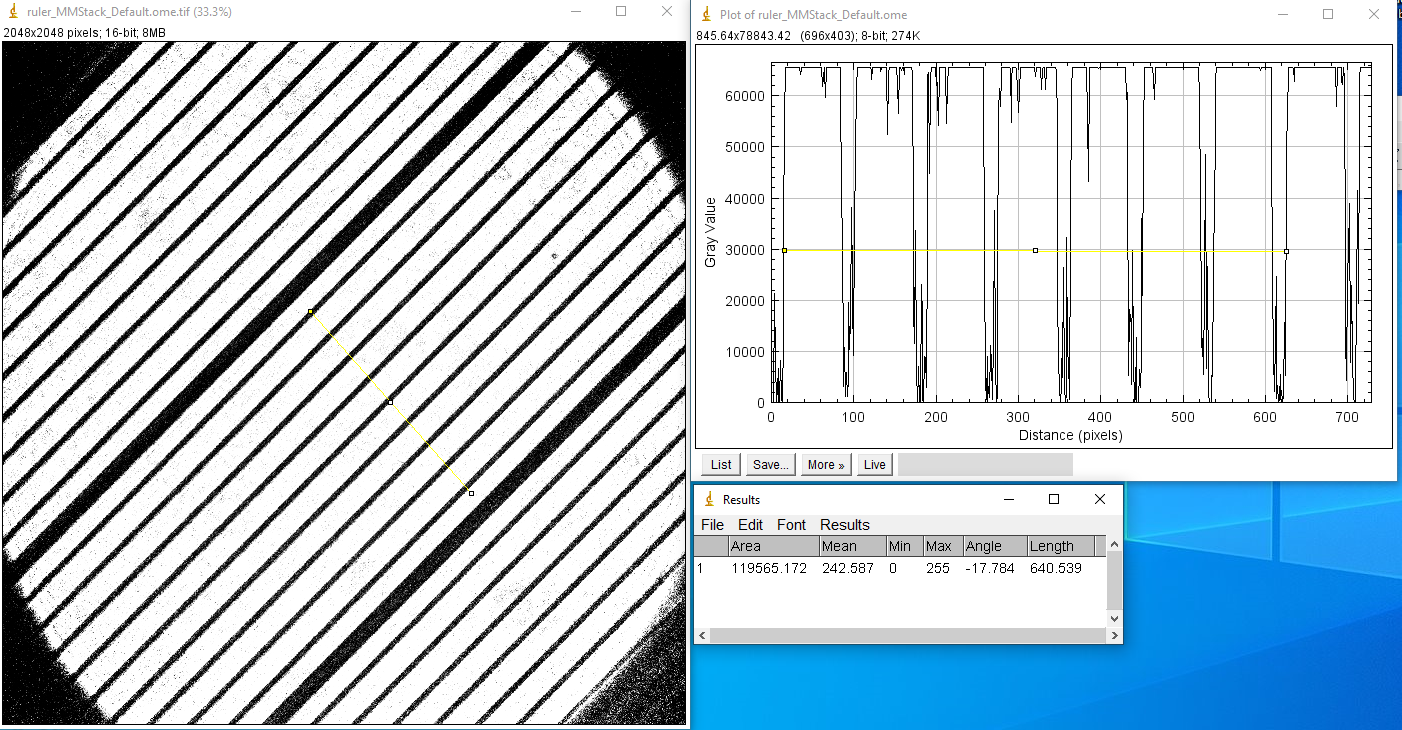
\includegraphics[width=0.9\textwidth]{Images/Ruler/measurements.png}
    \caption{Thorlabs 10 $\mu$m slides with ImageJ Analysis. The slides image was captured under the microscope and corrected color (left). A length (yellow line in the left picture) was selected and the grey value in this length was plotted (right top). Each high grey value area represents one small unit in the slides. The pixel size (right down) of selected region (yellow line in the right top) was measured to calculate the effective pixel values.}
    \label{fig:npc}
\end{figure}

Besides, the theoretical value of the effective pixel size could be determined from the optical instruments. If the camera pixel size is 6.5 µm and the magnification of the objective lens is 60x, the effective pixel size can be calculated as follows:

\[
\text{Effective Pixel Size} = \frac{\text{camera Pixel Size}}{\text{Objective magnification}} = \frac{ 6.5   \mu\text{m}}{ 60 \mu\text{m}} =  108.3\text{nm}
\]

Which matches our result.

\begin{comment}
To validate our result we can compute if the size of the real image on the slide corresponds to the size of the magnified image projected on the sensor. We use the known pixel size of our sensor ( 6.5 µm*6.5 µm) multiplied by the pixels under inquiry in Figure 2.1, divided by the real length of the scale in the image. 

\[
\text{Magnification} = \frac{\text{Projected Length}}{\text{Real Length}} = \frac{ 640.54 \text{pixels} * 6,5  \mu\text{m}}{ 70 \mu\text{m}} =  59.48x
\]

This actually suggests that the difference between the two methods to calculate the pixel size is caused by the magnification of the lens, which is rather 59,48x than the assumed 60x.
This can be confirmed even further by redoing the calculation with the effective magnification. and providing an even greater accordance between the two methods 1 \textperthousand  instead of 1 \% .
\[
\text{Effective Pixel Size} = \frac{\text{camera Pixel Size}}{\text{Objective magnification}} = \frac{ 6.5   \mu\text{m}}{ 59.48 \mu\text{m}} =  109.28 \text{nm}
\]
 This provides an even greater accordance between the two methods, giving an error of 1 \textperthousand instead of 1  \% .
\end{comment}xx


\section{Results}
%List the result of the four measurement as a chart
Figure 3.1 displayed the Nup96 nucleoporins reconstructed from the one of the movie recorded in the experiment. The movie was analyzed by thunderSTORM plugin, and elimated the drift by cross correlation method. The image of a single Nup96 nucleoporin is obtained with the same method and is shown in Figure 3.2. This procedure successfully visualized the octamer structure of Nup96 nucleoporins, allowing for a detailed analysis of the size and shape of the nuclear pore complexes in fixed U2OS cells. We selected five images and analyzed the distance between two Nup96 proteins (Table 3.1) and the diameter of the nuclear pore (Table 3.2).
  \begin{figure}[hbpt]
    \centering
    \begin{subfigure}[b]{0.45\textwidth}
        \centering
        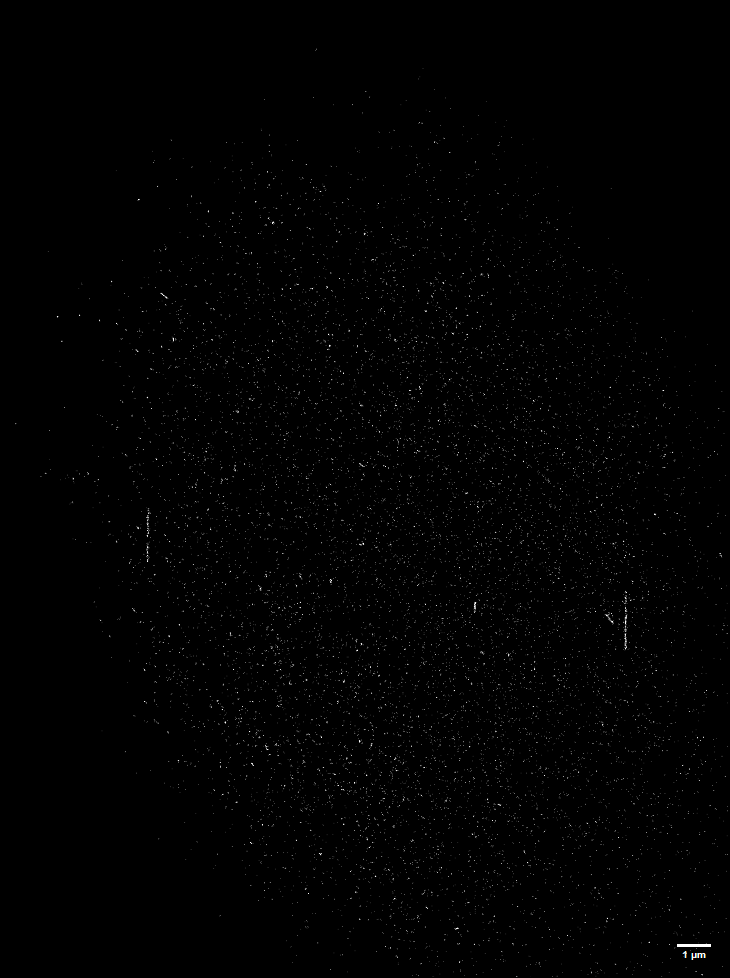
\includegraphics[width=\textwidth]{Images/STORM/5000frames.png}
        \caption{Reconstructed with 5000 frames}
        \label{fig:image1}
    \end{subfigure}
    \hfill
    \begin{subfigure}[b]{0.45\textwidth}
        \centering
        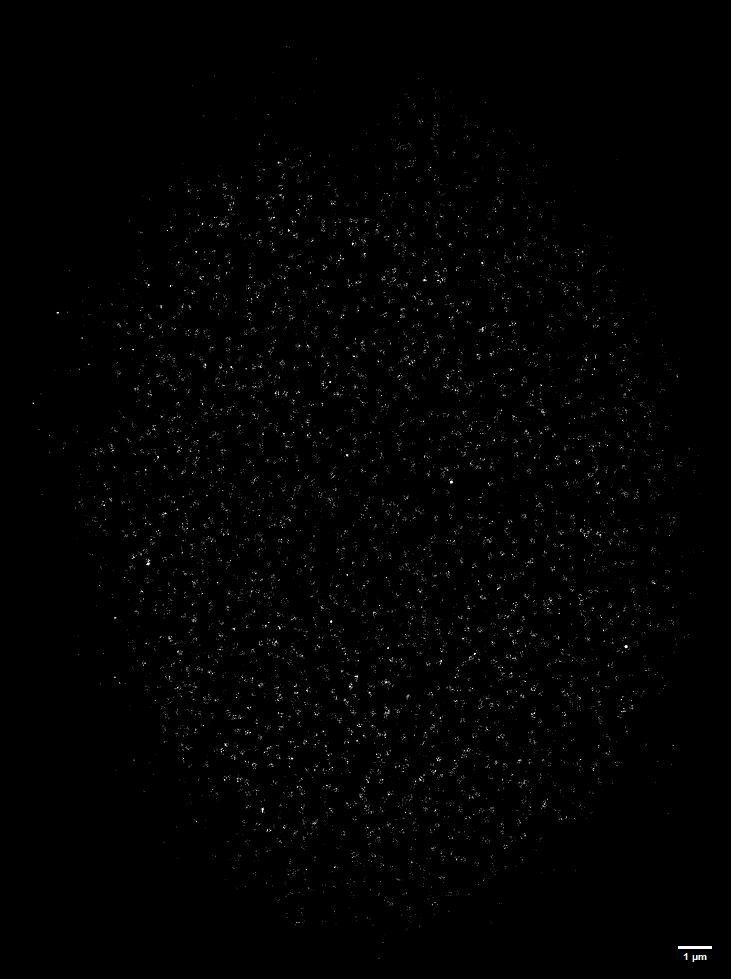
\includegraphics[width=\textwidth]{Images/STORM/10000frames.png}
        \caption{Reconstructed with 10000 frames}
        \label{fig:image2}
    \end{subfigure}
    \vfill
    \begin{subfigure}[b]{0.45\textwidth}
        \centering
        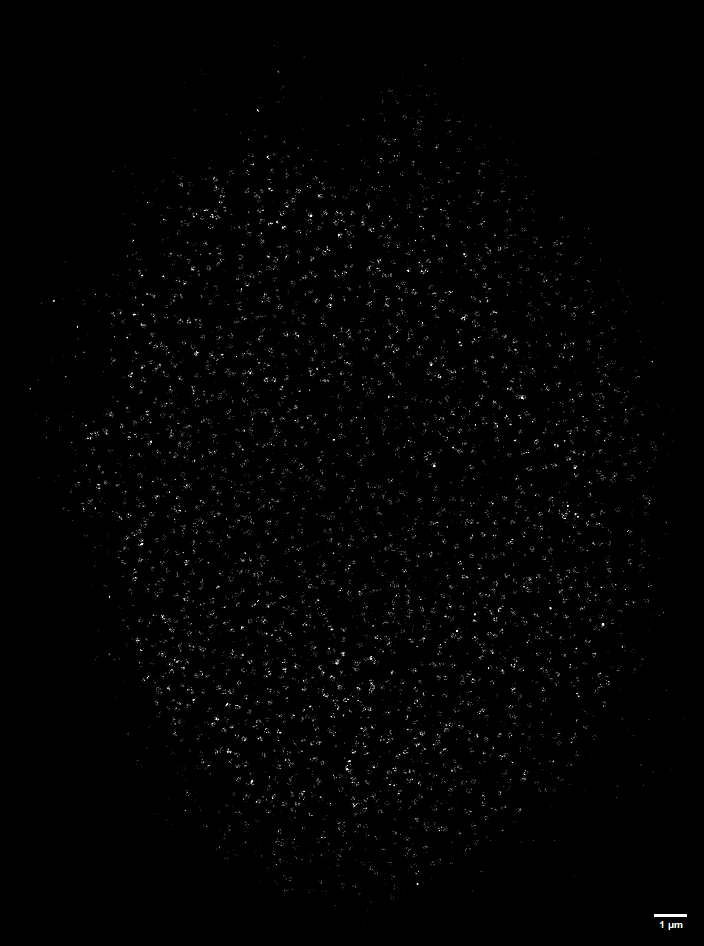
\includegraphics[width=\textwidth]{Images/STORM/20000frames.png}
        \caption{Reconstructed with 20000 frames}
        \label{fig:image3}
    \end{subfigure}
    \hfill
    \begin{subfigure}[b]{0.45\textwidth}
        \centering
        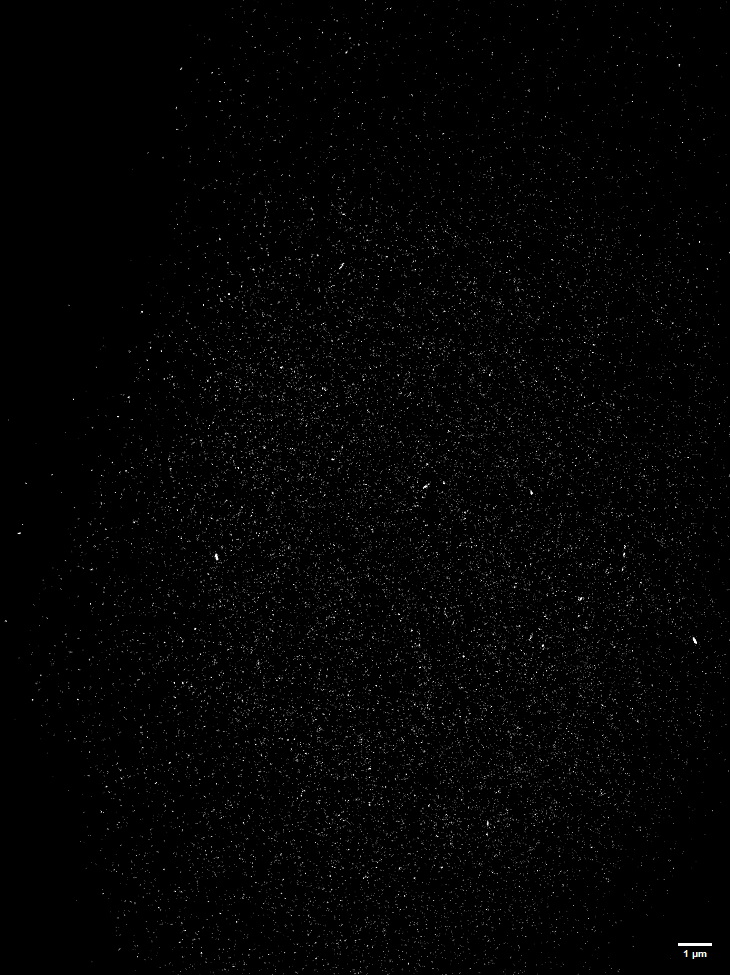
\includegraphics[width=\textwidth]{Images/STORM/20000frames20bins.png}
        \caption{Reconstructed with 20000 frames, bins=20}
        \label{fig:image4}
    \end{subfigure}
    \caption{The reconstructed nucleoporins Nup96 with different frames.(a), (b) and (c) are all reconstructed with same cross-correlation parameter(bins = 5).}
    \label{fig:subfigures}
\end{figure}

\begin{figure}
    \centering
    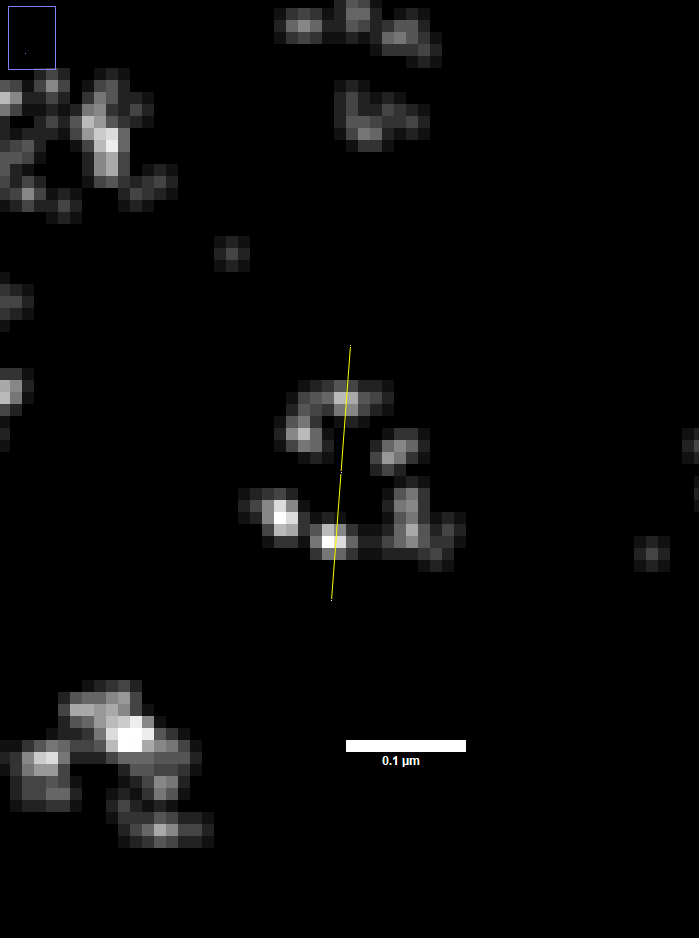
\includegraphics[width=0.5\linewidth]{Images/STORM/typical pore.png}
    \caption{The image of single Nup96 nucleoporin. The octamer structure could be observed.}
    \label{fig:enter-label}
\end{figure}
\begin{comment}
    \begin{figure}[h]
    \centering
    \begin{subfigure}[b]{0.45\textwidth}
        \centering
        \includegraphics[width=\textwidth]{image1.png}
        \caption{图片1标题}
        \label{fig:image1}
    \end{subfigure}
    \hfill
    \begin{subfigure}[b]{0.45\textwidth}
        \centering
        \includegraphics[width=\textwidth]{image2.png}
        \caption{图片2标题}
        \label{fig:image2}
    \end{subfigure}
    \vfill
    \begin{subfigure}[b]{0.45\textwidth}
        \centering
        \includegraphics[width=\textwidth]{image3.png}
        \caption{图片3标题}
        \label{fig:image3}
    \end{subfigure}
    \hfill
    \begin{subfigure}[b]{0.45\textwidth}
        \centering
        \includegraphics[width=\textwidth]{image4.png}
        \caption{图片4标题}
        \label{fig:image4}
    \end{subfigure}
    \caption{总标题}
    \label{fig:subfigures}
\end{figure}
\end{comment}

\begin{table}[hbpt]
    \centering
    \begin{tabular}{c|c|c}
    \hline
        Group & distance[nm]&fitted distance[nm] \\
    \hline
        1 &40.02 &44.85\\
        2 &69.56 &65.16\\
        3 &49.30 &51.26\\
        4 &49.48 &51.77\\
        5 &79.26 &75.08\\
    \hline
    \end{tabular}
    \caption{Distance between two Nup96 proteins, with average distance 57.52$\pm$ 16.25, and fitted average distance 57.62$\pm$ 12.24.}
    \label{tab:my_label}
\end{table}

\begin{table}[hbpt]
    \centering
    \begin{tabular}{c|c|c}
    \hline
        Group & diameter[nm]&fitted diameter[nm] \\
    \hline
        1 &108.99 &113.59\\
        2 &109.54 &111.85\\
        3 &108.64 &103.86\\
        4 &119.15 &122.17 \\
        5 &90.03 &100.33\\
        \hline
    \end{tabular}
    \caption{Diameter of the nuclear pore, with the average diameter 107.27 $\pm$ 10.59, and fitted average diameter 110.36 $\pm$ 8.59.}
    \label{tab:my_label}
\end{table}
\begin{comment}
dia
107.27000000000001 10.587022716514786
diaf
110.36000000000001 8.587490902469709
dis
57.524 16.248454695754916
disf
57.62399999999999 12.241814816439598


\end{comment}

\section{Discussion}
%Follow the script

Our analysis yielded an average diameter of 110.36 ± 8.59 nm for the Nup96 ring and an average distance of 57.62 ± 12.24 nm between adjacent Nup96 pairs. These values are somewhat larger than the expected literature values (107 nm \cite{nuclear_pores} and 42 nm\cite{nuclear_pores}, respectively). Several factors could contribute to these discrepancies:
a) Labeling strategy: The use of antibodies introduces additional size to the complex, potentially increasing the measured dimensions.
b) Localization precision: As with the nanoruler analysis, limitations in localization precision could lead to slight overestimations of distances.\\

 In figure 3.1, from (a) to (c), we observed that using the same cross correlation method with same bins, the resolution and the quality of figure is increasing with respect to the frame numbers, which is similar to the GATTAquant nanoruler experiment. And by changing the bins (d), the drift is much obvious than (c), indicating that the bins in the cross correlation are also an important parameter in the image analysis and drift elimination.\\

We acknowledge that some cherry-picking occurred in selecting figures for complete nuclear pores. This choice was motivated by two main factors:
a) The cells were subjected to harsh treatments during fixation and labeling, potentially damaging some protein complexes.
b) The inability to use active drift correction, as mentioned earlier, may have affected image quality for some nuclear pore complexes.\\

 It's worth noting that well-characterized point spread functions (PSFs) significantly enhance the confidence in determining the center of each fluorophore localization. We believe that the choice to use longer wavelengths (647 nm ) follows the consideration that longer wavelengths produce more spread-out PSFs, which are easier to characterize accurately on a sensor with limited. 
 
\printbibliography

\end{document}